% latex article template

% cheat sheet(eng): http://www.pvv.ntnu.no/~walle/latex/dokumentasjon/latexsheet.pdf
% cheat sheet2(eng): http://www.pvv.ntnu.no/~walle/latex/dokumentasjon/LaTeX-cheat-sheet.pdf
% reference manual(eng): http://ctan.uib.no/info/latex2e-help-texinfo/latex2e.html

% The document class defines the type of document. Presentation, article, letter, etc. 
\documentclass[12pt, a4paper]{article}

% packages to be used. needed to use images and such things. 
\usepackage[pdfborder=0 0 0]{hyperref}
\usepackage[utf8]{inputenc}
\usepackage[english]{babel}
\usepackage{graphicx}
\PassOptionsToPackage{hyphens}{url}

% hides the section numbering. 
\setcounter{secnumdepth}{-1}

% Graphics/image lications and extensions. 
\DeclareGraphicsExtensions{.pdf, .png, .jpg, .jpeg}
\graphicspath{{./images/}}

\title{
	Information systems\\
	project report\\	
}
\author{
	\underline{Group members:} \\
	Bae, Magnus\\
	Bremnes, Jan Alexander Stormark\\
	Krane, Magnus\\
	Sande, Kristian Olafsen\\
	Tørresen, Håvard\\
}
\date{\today}

\hypersetup{
	colorlinks=true,
	linkcolor=black,
	filecolor=red,
	urlcolor=blue
}

\begin{document}
\maketitle
\pagenumbering{arabic}

\newpage
\tableofcontents
\newpage
\section{Introduction}


This report documents the requirement specifications of “NTNUs Ultimate Digital Learning 
platform” (NUDL), which is a proposal for an IT-system for the Norwegian University of 
Science and Technology (NTNU). NUDL proposes to digitalize some of the current processes 
involved in studies at NTNU, such as delivering a complaint on a grade, to ease the 
process for all parties involved and cut an unnecessary load of paperwork. Beyond that 
it also proposes to streamline these processes, along with the processes that are 
already digitalized, under a standardized user interface and an updated security system.

\noindent
The report will begin with an analysis of the current situation, highlighting the 
processes and problems we found most in need of rework and digitalizing. Following, there 
will be an in-depth explanation of how we propose to solve these issues, and how NUDL 
will work and respond when put to use in situations that are managed by other systems 
today.

\section{Background}
In this chapter we will present the background for this project, and review the factors that have
influenced our decisions and vision for this project. %oldie incorporated into this one
\include{sections/analysis} %Old system goes here
\section{Our proposed solution}

%sleepy, can somebody proofread?
In this chapter we will discuss our proposed solution to the assignment and how we would like to digitalize NTNU's teaching processes. 

\subsection{What is wrong?}
Having initially looked at todays work processes we see lots of areas where things can be improved. Due to the limitations of this assignment not everything
is being pursued, but the idea behind our proposed solution is that it should be able to address all of the problems with the systems that are in use today. 

\noindent
Our biggest complaint about the current systems is that it's very fragmented and requires lots of labour-hours. There are, in our experience, discrepancies between what is 
stated on a webpage describing a subject, and what is the reality. Several of the group members have experienced being told ``we'll update it so it's correct for next year''. 
Staff have to keep their subjects updated in several places, there's course descriptions on NTNU webpages, there's It's Learning, and a lot of courses also have their own separate
web-page for those occasions where It's Learning doesn't cut it, or where they want to make information freely available. 

\noindent
Another problem seems to be the inherent problems with the technologies used. It's Learning tends to not learn a lot, but bugs both the users and itself with un-intuitive behaviour, 
odd bugs and browser incompatibility. For the last months logging into It's Learning has been messed up because it ends up just redirecting itself back to Innsida where one has to 
click once more (one group member even gets routed through It's Learning for HiST. It's Learning is for the most part a standalone system in a continuously more interconnected web full of ``open'' standards. The way we see it, It's Learning is the 
rod that has been pushed between the spokes of the wheel. There's a lot wrong with the system, but it's not all bad. It's just not right. In 2013 It's Learning is sadly holding the 
rest back. 

\subsection{What do we do?}
% http://www.ntnu.no/c/document_library/get_file?uuid=cc8a29fa-84f4-44b3-9af4-36e6c486746c&groupId=524136
% http://www.ntnu.no/c/document_library/get_file?uuid=ce1ba8c9-6744-42ff-bfe7-c114d58a36a6&groupId=524136
% file:///D:/Nedlastinger/Nettleser/hva_vet_vi_om_bruk_av_lms_i_uh-sektoren_4.ppt < "Evalueringer av LMS"
Based on our and others analysis we conclude that it's time to replace It's Learning. In the long term our plan is not only to replace It's Learning, but to create
a CMS\footnote{Content Managing System \url{https://en.wikipedia.org/wiki/Content_management_system}} and LMS\footnote{Learning Management System \url{https://en.wikipedia.org/wiki/Learning_management_system}} system that envelopes the whole of NTNU. It does sound very ambitious, but the plan is not to create a huge blob of software rather we propose a modularized tiered 
platform where data is stored in a centralized storage. The idea is to create a secure, robust, and manageable platform which is testable, modularized, and compartmentalized.
We also want to implement one thing that we really feel is missing today - search. 


Do you remember what was before Google? Yes, obviously you do, but do you remember how it really felt before Google? Maybe not so much. Search is good, but good search is better. 
According to Google Zeitgeist (search statistics) \cite{google:zeitgeist} people are to lazy to type in facebook.com, they just search for ``facebook''. Granted, the average NTNU 
student isn't your average person, but why should students have to manually navigate complex navigation trees when they can type a couple of words and get the result they want 
immediately? We think that by designing our system architecture and data storage with search in mind, we can bring value and help both students and staff to save time. 
\\\\
Today students have to interact with studentweb and It's Learning. Data gets passed one way only. We want our system to bridge the gap between the two by using a 
connector-pattern %lack of better name at the moment, can we come up with the right name for this pattern?
to link our system and FS/StudentWeb. This way, if one changes it's easy to adjust, and there is room for making our system better while the communication with FS is still bound by 
the same contract. We want to make our system interact with StudentWeb on part of the student. That means that the students interact with a system that is consistent. As a security 
measure our system will log error messages and calls, and in rare cases where propagation does not work as expected alerts can be raised and personel with the right clearances can 
take action and manually merge the discrepancy. %not sure about this last part(?)

\subsection{How do we do it}


\section{BPMN-models}
	The following BPMN-models\cite{bpmn} describe how we view the current processes of registering to a course, and complaining on a grade, followed by our suggested changes.
All models are from a student's perspective, as that is what we found most interesting.

\subsection{registering to a course}
		
\begin{figure}[H]
    \centering
    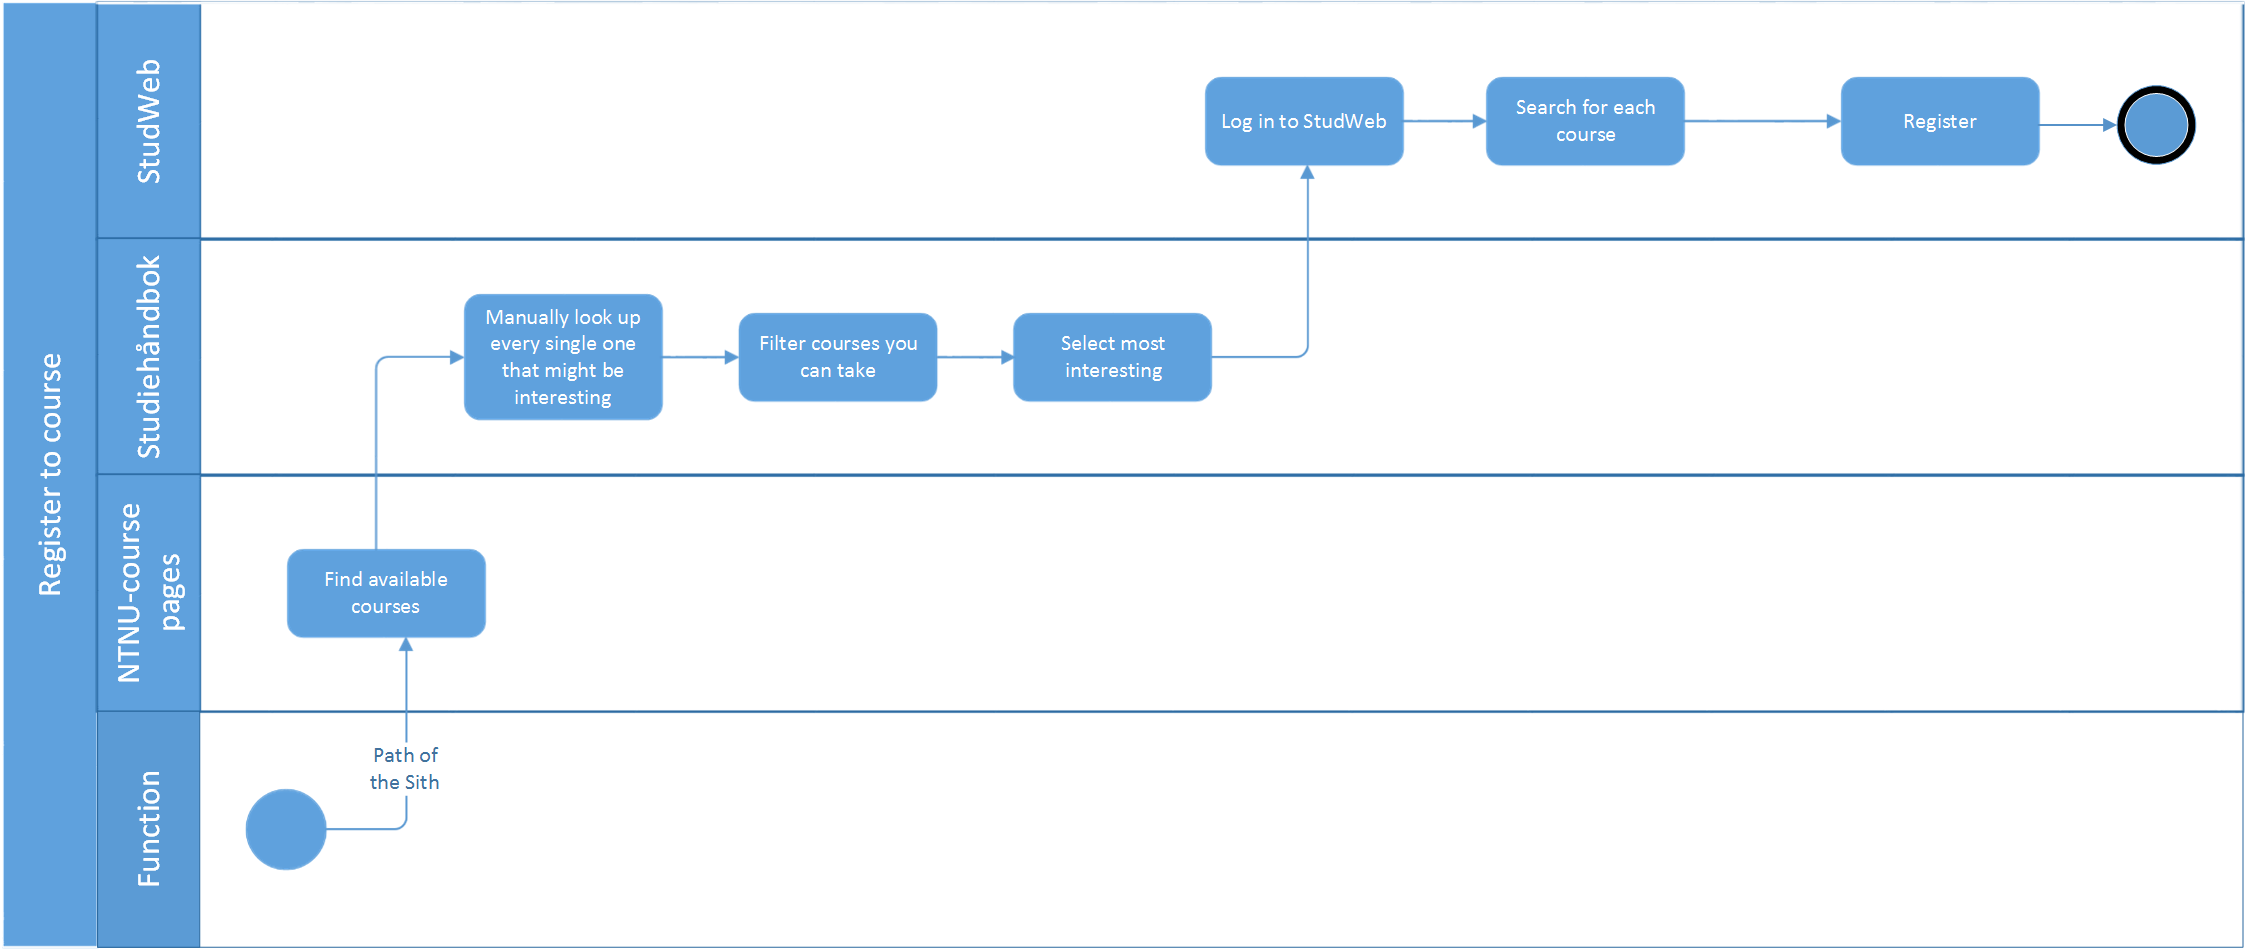
\includegraphics[width=\textheight, angle=-90]{BPMN-register-old}%apparently sets width first and then rotates
    \caption{Our interpretation of the current process of registering to a course.}
    \label{fig:Register-old}
\end{figure}

\begin{figure}[H]
    \centering
    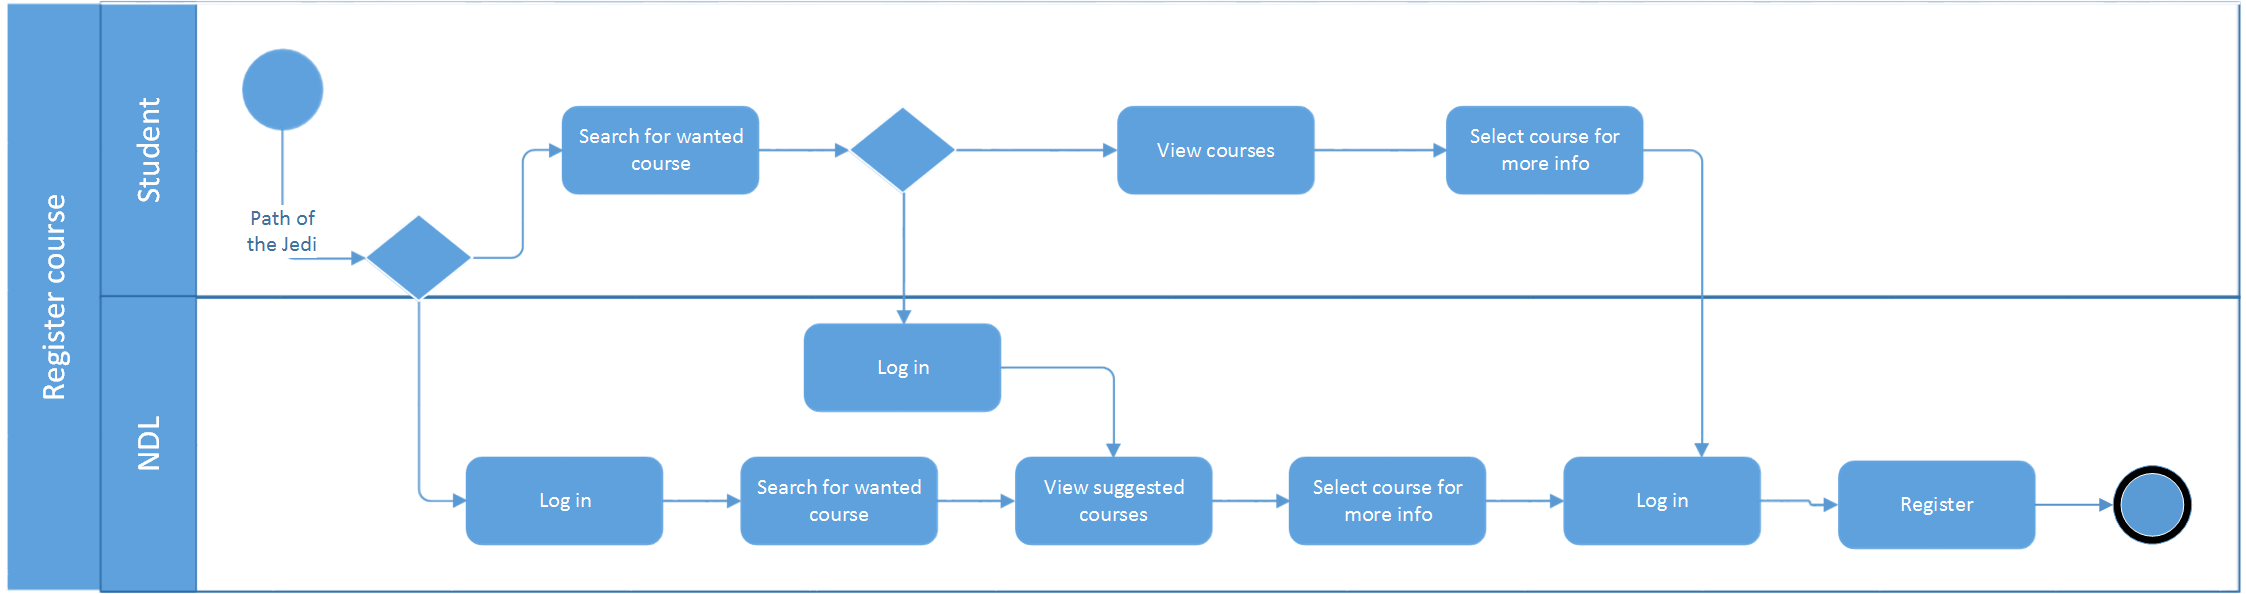
\includegraphics[width=\textheight, angle=-90]{BPMN-register}
    \caption{How we envision our new process of registering to a course to be.}
    \label{fig:Register-new}
\end{figure}

\begin{figure}[H]
    \centering
    \includegraphics[width=\textheight, angle=-90]{BPMN-complain-old}
    \caption{Our interpretation of the current process of complaining on a grade}
    \label{fig:Complain-old}
\end{figure}

\begin{figure}[H]
    \centering
    \includegraphics[width=\textheight, angle=-90]{BPMN-complain}
    \caption{How we envision our new process of complaining to be.}
    \label{fig:Complain-new}
\end{figure}
 % new system goes here
\section{How we are going to do it}
	This section will give a brief description of how we plan on implementing our solution. 
	
	\subsection{Central Datastore}
		We propose creating a central datastore containing all public information about NTNU. We will provide APIs that will give easy access to all the data, and the APIs will be open to the public. 
		% Tenk IME-API!
NUDL will use this datastore, illustrated in Figure \ref{fig:datastore}, to retrieve all necessary information about courses, rooms and timetables, and so it will need to be constantly updated in order to contain the most recent information. This means that third party developers will have equal access to non-restricted data, which will enable students and staff to write their own tools which can easily be integrated with NUDL. We aim to make NUDL a platform to which tools can be added and removed as needed, not a monolithic system where someone else is in control. The calendar generator at \url{www.ntnu.1024.no} is a great example of an extremely useful application created by a student. We know that IME offers some APIs today, and these could be extended and integrated into our system.
\begin{figure}[h]
\centering
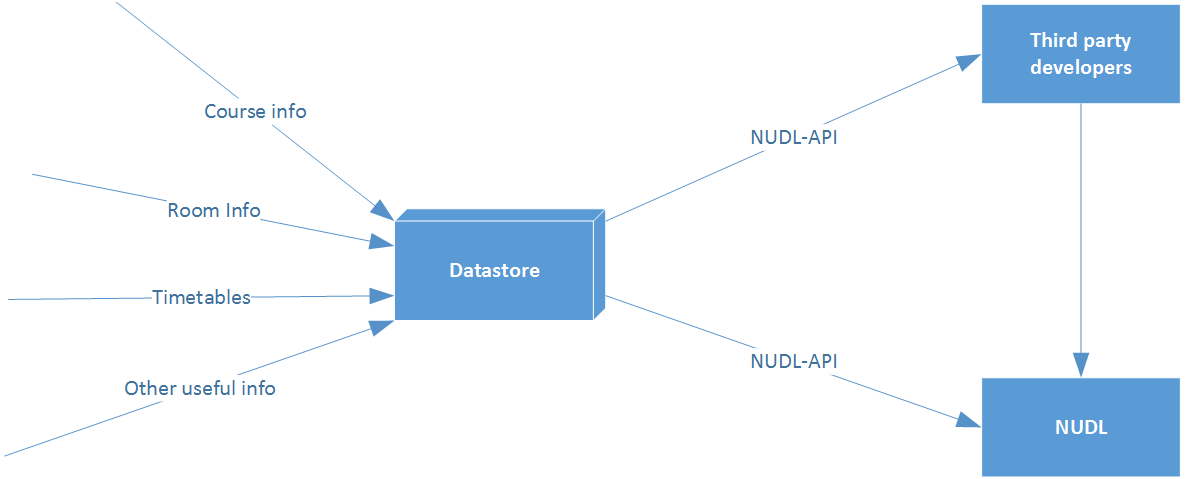
\includegraphics[width = \textwidth]{datastore}
\caption{Datastore and APIs}
\label{fig:datastore}
\end{figure}

	\subsection{Storage model}
		The datastore mentioned in the previous section will only contain publicly available information. In addition, we will have two other separate databases; one userstore containing information about staff and students, and one database storing everything related to the individual courses. In Figure \ref{fig:storagemodel} the general datastore is shown on the left, course database in the middle and userstore on the right. The dotted green circle means that everyone is given read access, a full red circle means read and write access is restricted to a strict subset of users, and a full green circle means that there are two different levels of security. The userstore will be fully secured against unauthorized access, and only the users will have access to their individual information. The course database will be used to supply the same functionality as It's Learning does today. Students will for the most part have read-only access to the course database, but they will be given the possibility to deliver exercises and participate in forums and chat. Course staff will have read and write access to the course content pages, but will only be able to read the student submissions. Administrative staff will have accesses as needed. 
Course staff will be able to make course material available to non-students, by making it accessible through the public APIs. 
\begin{figure}
\centering
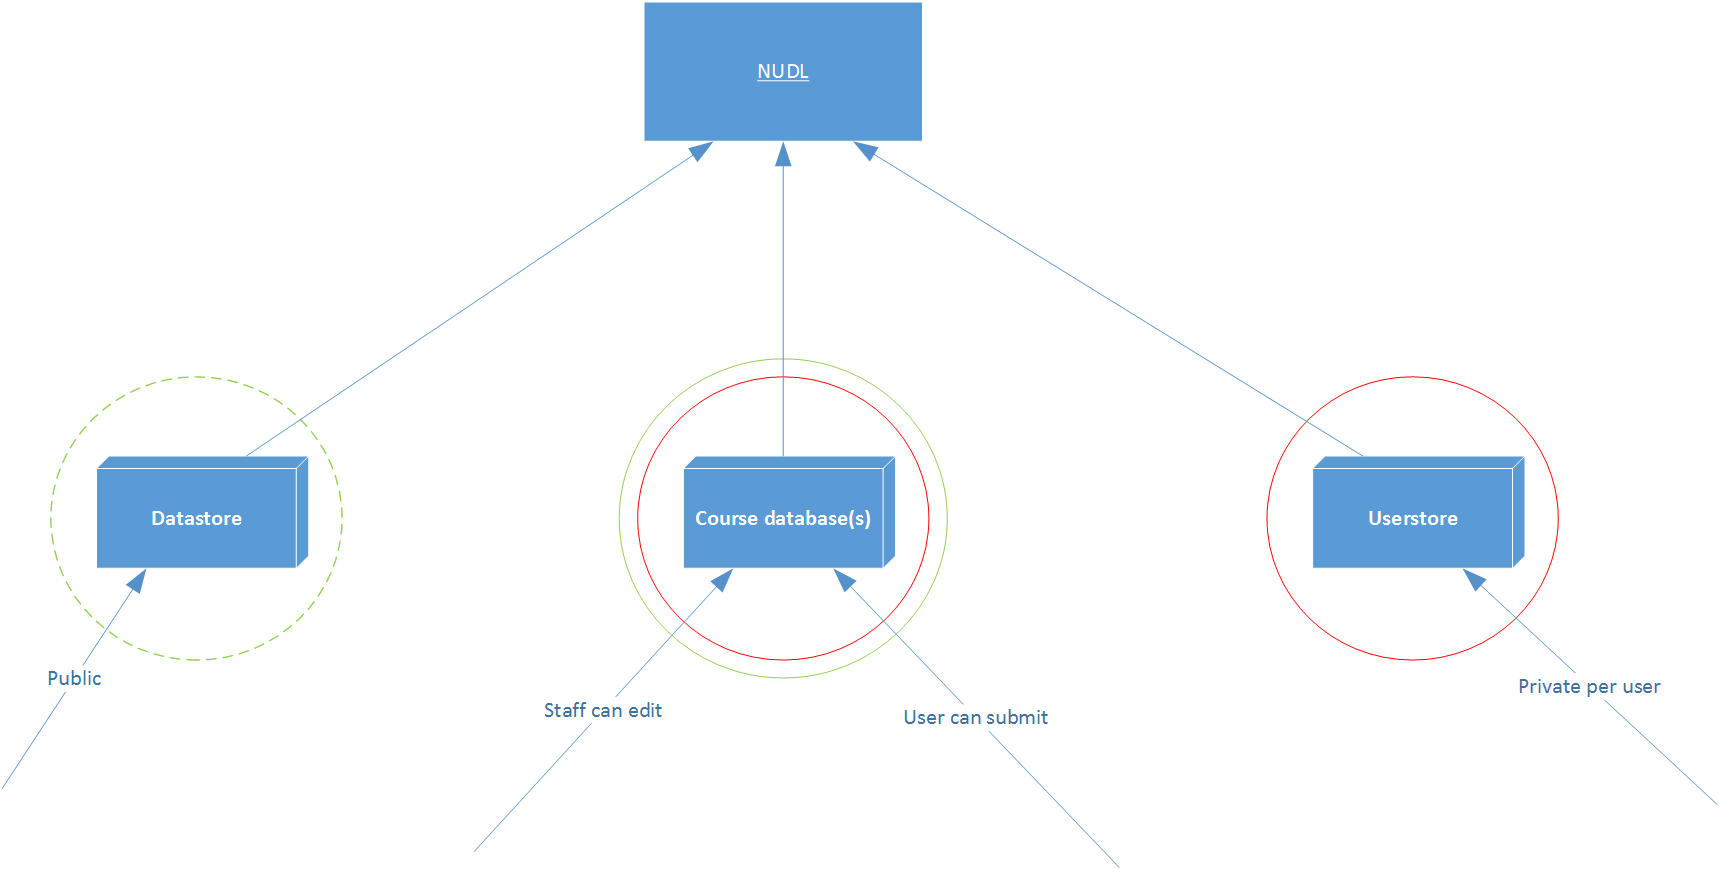
\includegraphics[width = \textwidth]{moreStorage}
\caption{Storage model}
\label{fig:storagemodel}
\end{figure}

		
	\subsection{User interface} 
		We want NUDL to present users with a user-friendly and unified interface. It will not be like today, where you have different interfaces for It's Learning, Studweb and Eksamensweb. It's Learning and Eksamensweb will be replaced by NUDL, and Studweb will be hidden from view. Students can log in to Studweb from NUDL, via Feide, but they will be met by the NUDL interface, which will take care of the communication with Studweb, as shown in Figure \ref{fig:layers}. Staff and students can do everything they need to do, from one central location. There will be no more need to log in to different services like today, where one first has to search for courses on ntnu.no, (UI no.1) log on to Studweb in order to register for the course (navigating a very cluttered and confusing UI no.2) and then log on to Innsida (UI no.3) and then finally continue to It's Learning (UI no.4). If they want to complain on a grade, they need to send in a paper form, or students at IDI can log on to Eksamensweb (UI no.5). NUDL combines all these different interfaces into one coherent whole. 
\begin{figure}
\centering
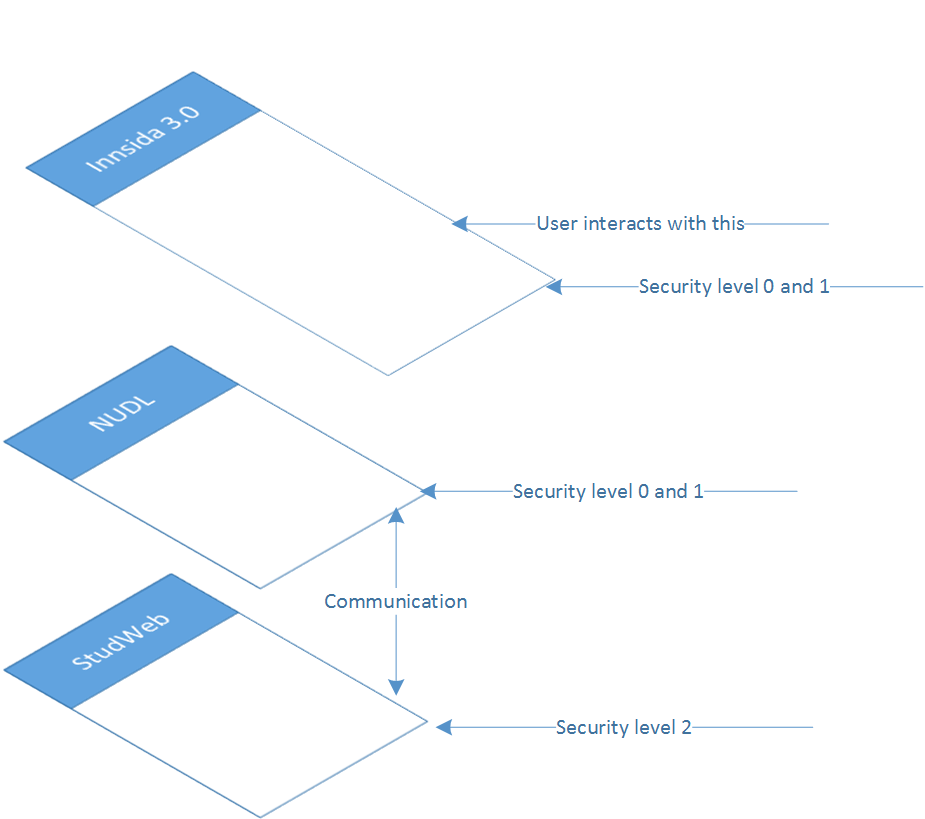
\includegraphics[width = \textwidth]{Layers}
\caption{Layered architecture}
\label{fig:layers}
\end{figure}

\bibliography{bibliography}
\bibliographystyle{acm}

\end{document}
